%%%%%%%%%%%%%%%%%%%%%%%%%%%%%%%%%%%%%%%%%%%%%%%%%%%%%%%%%%%%%%%%%%%%%%%%%%%%%%%
% SECTION: RESULTS (IEEE TSE Format) — Updated with Consolidated Results
%%%%%%%%%%%%%%%%%%%%%%%%%%%%%%%%%%%%%%%%%%%%%%%%%%%%%%%%%%%%%%%%%%%%%%%%%%%%%%%

% Note: Section header is in main_ieee_tse.tex

This section presents the experimental results organized by research questions.
The experiments address the four research questions defined in
Section~\ref{sec:experimental}, evaluating \filopriori{} across two
complementary datasets against five state-of-the-art deep learning baselines.

%------------------------------------------------------------------------------
% RQ1: Effectiveness on Industrial Dataset
%------------------------------------------------------------------------------

\subsection{RQ1: Effectiveness on Industrial Dataset}
\label{sec:rq1}

Table~\ref{tab:tcp_comparison} presents the comparison of \filopriori{} against
five deep learning baselines on the industrial QTA dataset (277 builds with at
least one failure). We use APFD as the primary metric with Wilcoxon signed-rank
tests for statistical significance.

\begin{table}[!t]
\centering
\caption{Comparison with Deep Learning Baselines (Industrial Dataset, 277 Builds)}
\label{tab:tcp_comparison}
\scriptsize
\begin{tabular}{lccccr}
\toprule
\textbf{Method} & \textbf{APFD} & \textbf{Std} & \textbf{p} & \textbf{$\delta$} & \textbf{$\Delta$} \\
\midrule
\textbf{\filopriori{}} & \textbf{0.761} & \textbf{0.189} & -- & -- & -- \\
DeepOrder~\cite{chen2023deeporder} & 0.689 & 0.266 & $<$0.001 & 0.10 (N) & +10.2\% \\
TCP-Net~\cite{abdelkarim2022tcp} & 0.670 & 0.271 & $<$0.001 & 0.14 (N) & +13.3\% \\
NodeRank~\cite{li2024noderank} & 0.661 & 0.270 & $<$0.001 & 0.14 (N) & +14.9\% \\
RETECS~\cite{spieker2017reinforcement} & 0.641 & 0.281 & $<$0.001 & 0.21 (S) & +18.6\% \\
FailRank-BB~\cite{hernandes2025method} & 0.595 & 0.263 & $<$0.001 & 0.35 (M) & +27.6\% \\
\bottomrule
\end{tabular}
\begin{tablenotes}
\small
\item *** $p < 0.001$ (Wilcoxon signed-rank test vs \filopriori{}).
\item $\delta$: Cliff's delta effect size. N = negligible ($<$0.147), S = small ($<$0.33),
M = medium ($<$0.474), L = large ($\geq$0.474)~\cite{arcuri2011practical}.
\item All methods evaluated on the same 277 builds with at least one failure.
\end{tablenotes}
\end{table}

\filopriori{} achieves a mean APFD of \textbf{0.7611} (std: 0.189),
outperforming all five deep learning baselines with statistical significance
($p < 0.001$). The improvements range from +10.2\% over DeepOrder (the
strongest baseline) to +27.6\% over FailRank-BB (the weakest).
Cliff's delta effect sizes range from negligible ($\delta = 0.10$, DeepOrder)
to medium ($\delta = 0.35$, FailRank-BB). The apparent discrepancy between
the large percentage improvements (+10.2\% to +27.6\% in mean APFD) and the
small-to-negligible per-build effect sizes reflects a fundamental difference
between the two measures: the percentage improvement captures the aggregate
shift in mean APFD across all 277 builds, while Cliff's delta measures how
often one method dominates the other on individual builds. A negligible
$\delta$ (e.g., 0.10 vs.\ DeepOrder) means that \filopriori{} outperforms
DeepOrder on only slightly more than half of the builds, but when it does
outperform, the APFD gains are substantially larger than the losses on the
builds where it underperforms, producing a meaningful shift in the mean.
This pattern is characteristic of TCP tasks with heavy-tailed build
distributions: a minority of builds with concentrated failures benefit
disproportionately from graph-based modeling, while simpler builds (with
few tests or obvious failure patterns) show little difference between methods.
The practical implication is that \filopriori{}'s advantage is concentrated on
the builds where prioritization matters most, specifically those with complex, non-trivial
failure patterns.

These results suggest that \filopriori{}'s multi-edge graph architecture effectively
exploits the rich structural information available in the
industrial dataset, even under strict temporal validation. DeepOrder and TCP-Net rely solely on historical features
without modeling relationships between test cases. RETECS, as a reinforcement
learning approach, struggles with the extreme sparsity of the reward signal inherent
in the 37:1 class imbalance, failing to optimize its ranking policy effectively. NodeRank,
while graph-based, relies on mutation sensitivity heuristics that are less effective at
isolating discriminative failure patterns than explicit message passing. FailRank-BB leverages semantic embeddings but relies on
Logistic Regression without graph-based modeling, which appears insufficient for
capturing the complex dependencies present in industrial test suites.

\textbf{Comparison with Heuristic Baselines.}
Table~\ref{tab:heuristic_industry} compares \filopriori{} against five
heuristic baselines on the industrial dataset. The strongest heuristic,
FailureRate (APFD = 0.664), outperforms Random (0.537) by a substantial
margin, confirming that historical failure patterns carry significant
predictive signal. However, \filopriori{} outperforms all heuristics by
at least +14.6\%, and the strongest deep learning baseline
(DeepOrder, APFD = 0.689) also exceeds all heuristics, validating our
choice to focus the main comparison on deep learning methods. Notably,
Recency (APFD = 0.420) performs \emph{below} random ordering on this
dataset. This contrasts with its strong performance on RTPTorrent
(Table~\ref{tab:rtptorrent_heuristic}), where recently\_failed achieves
0.821. The disparity is explained by the industrial test suite's
characteristics: with a 37:1 Pass:Fail ratio and long intervals between
failures for most tests, simple recency is a poor predictor; the more
informative signal comes from cumulative failure rates, which both
FailureRate and the deep learning baselines capture.

\begin{table}[!t]
\centering
\caption{Heuristic Baseline Comparison (Industrial Dataset, 277 Builds)}
\label{tab:heuristic_industry}
\scriptsize
\begin{tabular}{lccr}
\toprule
\textbf{Baseline} & \textbf{APFD} & \textbf{Std} & \textbf{$\Delta$ vs \filopriori{}} \\
\midrule
\textbf{\filopriori{}} & \textbf{0.761} & \textbf{0.189} & -- \\
FailureRate & 0.664 & 0.269 & +14.6\% \\
RecentFailureRate & 0.658 & 0.269 & +15.7\% \\
GreedyHistorical & 0.657 & 0.274 & +15.8\% \\
Random & 0.537 & 0.272 & +41.7\% \\
Recency & 0.420 & 0.313 & +81.2\% \\
\bottomrule
\end{tabular}
\begin{tablenotes}
\small
\item All heuristics use temporally accumulated history (no future leakage).
\item Recency ranks tests by builds since last failure. FailureRate
ranks by overall historical failure rate.
\end{tablenotes}
\end{table}

\textbf{Isolating Architectural vs.\ Balancing Contributions.}
A potential confound in the baseline comparison is that \filopriori{} uses a
different class-imbalance strategy (dual-balancing: balanced sampling at 29:1
+ focal loss) than the baselines, which use their native strategies. To
isolate whether \filopriori{}'s advantage stems from the GATv2 graph
architecture or from the balancing strategy, we retrained DeepOrder (the
strongest baseline, APFD = 0.689) using \filopriori{}'s dual-balancing
protocol, keeping all other aspects of DeepOrder unchanged (same 8 features,
same network architecture, same evaluation).
Table~\ref{tab:deeporder_dualbalancing} presents the results.

\begin{table}[!t]
\centering
\caption{Isolating Architectural vs.\ Balancing Contributions (Industrial
Dataset). DeepOrder retrained with \filopriori{}'s dual-balancing strategy.}
\label{tab:deeporder_dualbalancing}
\footnotesize
\begin{tabular}{lcc}
\toprule
\textbf{Configuration} & \textbf{APFD} & \textbf{$\Delta$ vs \filopriori{}} \\
\midrule
\filopriori{} (Full) & 0.761 & -- \\
\filopriori{} w/o Dual-Balancing & 0.729 & $-$4.0\% \\
\midrule
DeepOrder (original BCE) & 0.689 & $-$9.4\% \\
DeepOrder + Balanced Sampling & 0.687 & $-$9.7\% \\
DeepOrder + Dual-Balancing & 0.676 & $-$11.3\% \\
\bottomrule
\end{tabular}
\begin{tablenotes}
\small
\item Dual-Balancing = Balanced Sampling (29:1) + Focal Loss ($\alpha_f\!=\!0.75$, $\gamma\!=\!2.0$).
\item All configurations use the same 277 test builds and identical evaluation protocol.
\end{tablenotes}
\end{table}

DeepOrder with \filopriori{}'s dual-balancing achieves APFD = 0.676,
\emph{below} its original score (0.689, $-$1.9\%), and 11.3\% below
\filopriori{} (0.761). The balanced-sampling-only variant (0.687) is also
marginally below the original. This demonstrates that \filopriori{}'s
balancing strategy is not transferable to DeepOrder's architecture:
the dual-balancing was co-optimized with the GATv2 architecture, and
applying it to a flat-feature DNN slightly disrupts its native training
dynamics. Crucially, the 9.7\% gap between the best DeepOrder variant
(0.687) and \filopriori{} (0.761) is primarily attributable to the GATv2
graph architecture, confirming that the graph-based structural modeling
provides genuine advantages beyond class-imbalance handling.

%------------------------------------------------------------------------------
% RQ1: Effectiveness on RTPTorrent
%------------------------------------------------------------------------------

\subsection{RQ1: Effectiveness on RTPTorrent}
\label{sec:rq1_rtptorrent}

To evaluate generalization across diverse open-source projects, we
conducted experiments on the RTPTorrent benchmark~\cite{mattis2020rtptorrent},
which contains test execution histories from 20 Java projects with over 100,000
Travis CI builds. We evaluated \filopriori{} using its ensemble architecture
(Section~\ref{sec:ensemble}), trained independently on each project.

\textbf{Comparison with Deep Learning Baselines.}
Table~\ref{tab:rtptorrent_dl} presents the aggregate results of \filopriori{}
against the five deep learning baselines on the RTPTorrent dataset.

\begin{table}[!t]
\centering
\caption{Deep Learning Baseline Comparison (RTPTorrent, 20 Projects)}
\label{tab:rtptorrent_dl}
\scriptsize
\begin{tabular}{lcccccr}
\toprule
\textbf{Method} & \textbf{APFD} & \textbf{Std} & \textbf{N} & \textbf{p} & \textbf{$\delta$} & \textbf{$\Delta$} \\
\midrule
\textbf{\filopriori{}} & \textbf{0.854} & \textbf{0.111} & 2,937 & -- & -- & -- \\
TCP-Net~\cite{abdelkarim2022tcp} & 0.825 & 0.110 & 2,937 & 0.087 & 0.08 (N) & +1.6\% \\
FailRank-BB~\cite{hernandes2025method} & 0.822 & 0.092 & 2,937 & 0.046* & 0.15 (S) & +2.0\% \\
DeepOrder~\cite{chen2023deeporder} & 0.814 & 0.104 & 2,937 & 0.018* & 0.16 (S) & +3.0\% \\
NodeRank~\cite{li2024noderank} & 0.809 & 0.114 & 2,937 & 0.009** & 0.20 (S) & +5.6\% \\
RETECS~\cite{spieker2017reinforcement} & 0.679 & 0.156 & 2,937 & $<$0.001 & 0.65 (L) & +23.5\% \\
\bottomrule
\end{tabular}
\begin{tablenotes}
\small
\item Grand mean APFD computed as the average of 20 per-project mean APFD values.
\item Wilcoxon signed-rank tests and Cliff's $\delta$ computed on the 20 paired per-project means ($n = 20$).
\item $\delta$: Cliff's delta. N = negligible, S = small, M = medium, L = large~\cite{arcuri2011practical}.
\item All methods evaluated on the same 2,937 builds with failures across 20 projects.
\end{tablenotes}
\end{table}

\filopriori{} achieves the highest aggregate APFD (0.8540) among all
evaluated methods, with statistically significant improvements over four of
five deep learning baselines: FailRank-BB (+2.0\%, $p=0.046$), DeepOrder
(+3.0\%, $p=0.018$), NodeRank (+5.6\%, $p=0.009$), and RETECS (+23.5\%,
$p<0.001$). The difference from TCP-Net (+1.6\%, $p=0.087$) does not reach
statistical significance at $\alpha=0.05$.

\textbf{Multiple-comparison correction.} Applying Holm-Bonferroni correction
to the five pairwise comparisons renders the differences from TCP-Net
($p=0.087$, not significant before correction) and FailRank-BB ($p=0.046$,
adjusted $\approx 0.18$) non-significant. DeepOrder ($p=0.018$, adjusted
$\approx 0.054$) is marginal. Only NodeRank ($p=0.009$) and RETECS
($p<0.001$) remain significant after correction. The RTPTorrent results
show that \filopriori{} achieves the numerically highest APFD with
statistically robust improvements over NodeRank and RETECS, while the
differences from TCP-Net, FailRank-BB, and DeepOrder should be interpreted
with caution.

Cliff's delta effect sizes on the 20 paired per-project means confirm
these patterns: the effect vs.\ RETECS is large ($\delta = 0.65$),
vs.\ NodeRank and DeepOrder small ($\delta = 0.20$ and $0.16$),
and vs.\ TCP-Net negligible ($\delta = 0.08$) and vs.\ FailRank-BB small ($\delta = 0.15$).
These small-to-negligible effect sizes for the top baselines,
combined with the limited statistical power ($n = 20$ paired observations),
are consistent with the multiple-comparison analysis above.
The reduced margin relative to the industrial dataset is consistent with the
limited semantic information available in RTPTorrent (test names only, no
descriptions or commits), which constrains the advantage of \filopriori{}'s
semantic stream.

\textbf{Comparison with Heuristic Baselines.}
Table~\ref{tab:rtptorrent_heuristic} compares \filopriori{} against the
standard heuristic baselines provided with the RTPTorrent benchmark.

\begin{table}[!t]
\centering
\caption{Heuristic Baseline Comparison (RTPTorrent, 20 Projects)}
\label{tab:rtptorrent_heuristic}
\scriptsize
\begin{tabular}{lccr}
\toprule
\textbf{Baseline} & \textbf{APFD} & \textbf{$\Delta$ vs \filopriori{}} & \textbf{p-value} \\
\midrule
optimal\_failure (oracle) & 0.9249 & -9.3\% & -- \\
\textbf{\filopriori{}} & \textbf{0.8540} & -- & -- \\
recently\_failed & 0.8209 & +2.1\% & sig.* \\
optimal\_duration & 0.5934 & +41.3\% & $<$0.001*** \\
matrix\_naive & 0.5693 & +47.3\% & $<$0.001*** \\
random & 0.4940 & +69.7\% & $<$0.001*** \\
matrix\_conditional & 0.5132 & +63.4\% & $<$0.001*** \\
untreated & 0.3574 & +134.5\% & $<$0.001*** \\
\bottomrule
\end{tabular}
\begin{tablenotes}
\small
\item Aggregate results over 2,937 test builds from 20 Java projects.
\item * Statistically significant improvement over strongest heuristic baseline.
\end{tablenotes}
\end{table}

\filopriori{} surpasses all heuristic baselines except the oracle
(optimal\_failure), which requires perfect failure knowledge. The improvement
over the strongest heuristic (recently\_failed) is +2.1\%, while the
improvement over random ordering is +69.7\%.

\textbf{Per-Project Analysis.}
Table~\ref{tab:rtptorrent_perproject} presents the per-project APFD for
\filopriori{} and the five deep learning baselines across all 20 RTPTorrent
projects.

\begin{table*}[!t]
\centering
\caption{Per-Project APFD Comparison (RTPTorrent, 20 Projects, Ensemble Variant). Bold indicates the best method for each project.}
\label{tab:rtptorrent_perproject}
\footnotesize
\begin{tabular}{lcccccc}
\toprule
\textbf{Project} & \textbf{\filopriori{}} & \textbf{TCP-Net} & \textbf{FailRank-BB} & \textbf{DeepOrder} & \textbf{NodeRank} & \textbf{RETECS} \\
\midrule
facebook/buck & \textbf{0.9831} & 0.9149 & 0.9125 & 0.8683 & 0.9792 & 0.7437 \\
apache/sling & \textbf{0.9710} & 0.9589 & 0.9427 & 0.9320 & 0.9540 & 0.8385 \\
eclipse/jetty.project & \textbf{0.9719} & 0.9673 & 0.9487 & 0.9463 & 0.9702 & 0.9103 \\
jOOQ/jOOQ & \textbf{0.9392} & 0.9311 & 0.9250 & 0.9262 & 0.9316 & 0.7755 \\
julianhyde/optiq & 0.9135 & 0.9122 & 0.8987 & \textbf{0.9208} & 0.9058 & 0.8321 \\
jcabi/jcabi-github & \textbf{0.9370} & 0.8431 & 0.8704 & 0.7809 & 0.8576 & 0.6513 \\
CloudifySource/cloudify & 0.9086 & \textbf{0.9096} & 0.8731 & 0.8994 & 0.7481 & 0.7903 \\
square/okhttp & \textbf{0.8916} & 0.8679 & 0.8680 & 0.8258 & 0.8499 & 0.7909 \\
Graylog2/graylog2-server & \textbf{0.8940} & 0.8585 & 0.7708 & 0.8817 & 0.8837 & 0.4312 \\
doanduyhai/Achilles & \textbf{0.8693} & 0.8242 & 0.7739 & 0.8135 & 0.7817 & 0.7040 \\
SonarSource/sonarqube & \textbf{0.8671} & 0.8371 & 0.6934 & 0.7964 & 0.8150 & 0.7680 \\
thinkaurelius/titan & \textbf{0.8410} & 0.8394 & 0.8350 & 0.8441 & 0.8003 & 0.7371 \\
deeplearning4j/dl4j & 0.8361 & 0.8369 & \textbf{0.8428} & 0.8330 & 0.8049 & 0.7480 \\
jsprit/jsprit & 0.9426 & \textbf{0.9586} & 0.8959 & 0.9305 & 0.9109 & 0.6215 \\
dynjs/dynjs & 0.8001 & 0.6961 & \textbf{0.8294} & 0.7777 & 0.7285 & 0.4948 \\
adamfisk/LittleProxy & 0.7196 & 0.7302 & \textbf{0.7807} & 0.6718 & 0.6879 & 0.5742 \\
neuland/jade4j & 0.7239 & 0.7285 & 0.7141 & \textbf{0.7307} & 0.6765 & 0.5901 \\
brettwooldridge/HikariCP & 0.6616 & 0.6497 & \textbf{0.7520} & 0.6687 & 0.6444 & 0.5685 \\
DSpace/DSpace & 0.6841 & 0.6425 & \textbf{0.7027} & 0.6353 & 0.6521 & 0.4065 \\
l0rdn1kk0n/wicket-bootstrap & 0.5971 & 0.5993 & \textbf{0.6056} & 0.5896 & 0.5985 & \textbf{0.6056} \\
\midrule
\textbf{Grand Mean} & \textbf{0.8540} & 0.8253 & 0.8218 & 0.8136 & 0.8090 & 0.6791 \\
\bottomrule
\end{tabular}
\end{table*}

\filopriori{} achieves the highest APFD in \textbf{11 out of 20 projects},
with particularly strong performance on projects with rich failure
histories and consistent failure patterns (e.g., facebook/buck: 0.9831,
apache/sling: 0.9710, eclipse/jetty.project: 0.9719).

\filopriori{} underperforms on two projects relative to the strongest baselines:
jsprit/jsprit (0.9426 vs TCP-Net's 0.9586) and dynjs/dynjs (0.8001 vs
FailRank-BB's 0.8294). These projects share common characteristics: very sparse
failure data (10 and 11 builds with failures, respectively) and high variance
in failure patterns. In these scenarios with limited evaluation data,
the statistical reliability of the APFD estimates is reduced. We discuss
these cases further in Section~\ref{sec:discussion}.

Figure~\ref{fig:apfd_comparison} provides a visual comparison of all methods
across both datasets, highlighting the different competitive landscapes:
large margins on the industrial dataset (where graph-based modeling dominates)
and narrow margins on RTPTorrent (where the DNN ensemble compensates for
sparse metadata).

\begin{figure}[!t]
    \centering
    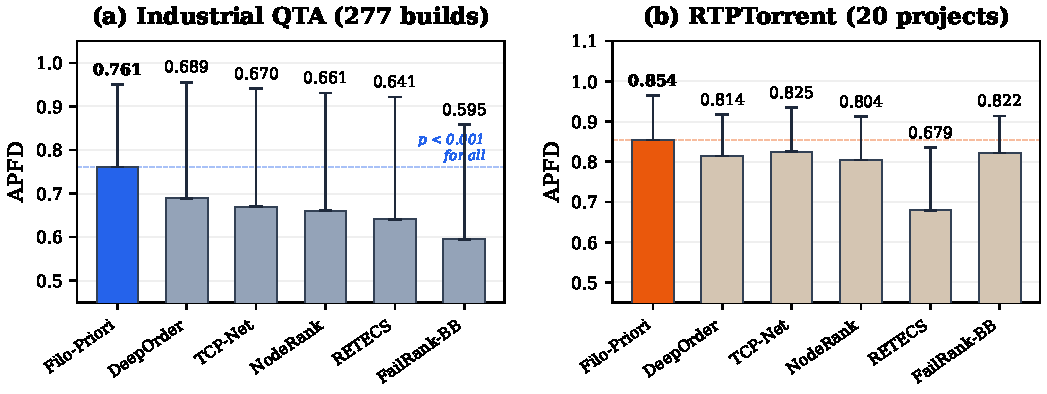
\includegraphics[width=\columnwidth]{figures/fig_apfd_comparison.pdf}
    \caption{Cross-dataset APFD comparison. \filopriori{} (dark bars) achieves
    the highest APFD on both datasets. Error bars show standard deviation
    across builds (industrial) or projects (RTPTorrent). The competitive
    landscape differs substantially: large margins on the industrial dataset
    ($+10$--$28\%$, $p<0.001$) vs.\ narrow margins on RTPTorrent.}
    \label{fig:apfd_comparison}
\end{figure}

\textbf{Semantic Signal Analysis: Identity Proxy Effect.}
FailRank-BB's competitive performance on RTPTorrent (0.822, third place)
despite using only SBERT embeddings of test names (no historical
features, no commit data) appears to contradict the finding that semantic
features do not contribute to TCP. To investigate this apparent
contradiction, we conducted a controlled experiment that disentangles
the semantic content of embeddings from their role as test case
identifiers.

We evaluated FailRank-BB under three embedding conditions on all 20
RTPTorrent projects: (1)~\textbf{SBERT}: the original configuration with
real Sentence-BERT embeddings of test names; (2)~\textbf{Random-Fixed}:
each test name is assigned a random 768-dimensional vector, but the
same random vector is used consistently across all builds for the
same test (preserving identity without semantic content); and
(3)~\textbf{Random-Shuffled}: fresh random vectors are generated for each
test in each build (destroying both semantic content and identity signal).
Table~\ref{tab:semantic_control} presents the results.

\begin{table}[!t]
\centering
\caption{Semantic Signal Control Experiment (RTPTorrent, 20 Projects).
Embedding conditions vary the information available to FailRank-BB's
Logistic Regression classifier.}
\label{tab:semantic_control}
\footnotesize
\begin{tabular}{lccl}
\toprule
\textbf{Condition} & \textbf{APFD} & \textbf{Std} & \textbf{Signal} \\
\midrule
Random-Fixed & 0.856 & 0.095 & Identity only \\
SBERT (original) & 0.822 & 0.092 & Identity + semantics \\
Random-Shuffled & 0.514 & 0.063 & None (random baseline) \\
\bottomrule
\end{tabular}
\begin{tablenotes}
\small
\item Random-Fixed assigns a consistent random vector per test name.
\item Random-Shuffled generates fresh random vectors each build.
\item All conditions use the same LogisticRegression classifier and
temporal split as the original FailRank-BB experiment.
\end{tablenotes}
\end{table}

The results are unambiguous. Random-Fixed embeddings (0.856) outperform
real SBERT embeddings (0.822), demonstrating that semantic content in test
names does not contribute to FailRank-BB's effectiveness; in fact, it
slightly degrades performance. The critical factor is identity
consistency: any fixed vector that uniquely identifies a test case allows
the Logistic Regression to learn per-test failure rates from the training
data. When this identity signal is destroyed (Random-Shuffled), performance
collapses to the random baseline (0.514). FailRank-BB is therefore
functionally equivalent to a per-test failure rate lookup table, not a
semantic model, and its competitive RTPTorrent performance does not
constitute evidence for the value of semantic features in TCP. This finding
is discussed further in Section~\ref{sec:discussion}.

\textbf{Identity Proxy Test on \filopriori{}'s Semantic Stream.}
To complete the identity proxy analysis, we applied the same Random-Fixed
control to \filopriori{} itself on the industrial dataset. We replaced the
SBERT embeddings in the semantic stream with hash-seeded random vectors
(consistent per test case across builds), keeping all other components
identical (GATv2, structural features, graph construction, training
strategy). Table~\ref{tab:filopriori_randomfixed} presents the results.

\begin{table}[!t]
\centering
\caption{Identity Proxy Test on \filopriori{}'s Semantic Stream (Industrial
Dataset, 277 Builds). Random-Fixed embeddings replace SBERT in the semantic
stream only; all other components unchanged.}
\label{tab:filopriori_randomfixed}
\footnotesize
\begin{tabular}{lccl}
\toprule
\textbf{Embedding} & \textbf{APFD} & \textbf{$\Delta$} & \textbf{Interpretation} \\
\midrule
SBERT (original) & 0.756 & -- & Full model \\
Random-Fixed & 0.756 & $+$0.0\% & Identity proxy test \\
\bottomrule
\end{tabular}
\begin{tablenotes}
\small
\item Random-Fixed assigns a deterministic random 1536-dim vector per TC\_Key.
\item Same graph, structural features, and training protocol as the validated experiment.
\item Wilcoxon signed-rank test on 277 paired per-build APFD values: $p = 0.965$.
\end{tablenotes}
\end{table}

Random-Fixed embeddings achieve APFD = 0.756, statistically
indistinguishable from the SBERT baseline (0.756, $p = 0.965$, Cliff's
$\delta = 0.013$, negligible). This confirms that \filopriori{}'s semantic
stream, like FailRank-BB's (Table~\ref{tab:semantic_control}), exploits
embedding consistency as an identity proxy rather than semantic content.
The 19 structural features and GATv2 graph attention subsume any
discriminative signal that generic sentence embeddings provide, and
replacing them with random but consistent vectors produces identical
prioritization effectiveness.

%------------------------------------------------------------------------------
% RQ2: Component Contributions
%------------------------------------------------------------------------------

\subsection{RQ2: Ablation Study}
\label{sec:rq2}

To understand the contribution of each architectural component, we conducted
a systematic ablation study on the industrial dataset. The ablation follows
a strictly subtractive protocol: starting from the full
\textsc{Filo-Priori-Full} model (APFD = 0.7611), we remove one component at
a time and measure the resulting performance degradation. This isolates the
marginal contribution of each component within the complete system.

\textbf{Baseline Architecture Definition.}
It is the dual-stream GATv2 model stripped of
the five innovations evaluated in the ablation: it uses a co-failure-only
graph (no multi-edge extension), has no orphan KNN scoring pipeline, uses the
original triple-compensation balancing strategy instead of the simplified
dual-balancing approach, uses the default classification threshold (0.50),
and excludes the nine DeepOrder-inspired temporal features (retaining only
the 10 base structural features). This baseline represents the core GATv2
architecture before the innovations introduced in this work.
The Baseline Architecture achieves APFD = 0.6503 in the full-system
ablation (Table~\ref{tab:ablation}) and APFD = 0.6397 in the
component-isolation analysis (Table~\ref{tab:ablation_isolation}). The
1.6\% difference arises because the two analyses use different starting
points: Table~\ref{tab:ablation} removes components from the full model
(subtractive), while Table~\ref{tab:ablation_isolation} removes components
from the baseline itself (isolation), resulting in different interaction
effects between components.

Table~\ref{tab:ablation} presents the full-system ablation: each row removes
one component from the complete model. Table~\ref{tab:ablation_isolation}
presents a complementary component-isolation analysis where each variant is
evaluated from the baseline upward.

\begin{table}[!t]
\centering
\caption{Ablation Study: Component Contributions (Industrial Dataset)}
\label{tab:ablation}
\begin{tabular}{lccc}
\toprule
\textbf{Configuration} & \textbf{APFD} & \textbf{$\Delta$} & \textbf{p-value} \\
\midrule
Full Model & 0.7611 & -- & -- \\
\midrule
w/o Enriched Multi-Edge Graph & 0.6835 & -10.0\% & $<$0.001*** \\
w/o Orphan KNN Scoring & 0.7145 & -5.9\% & $<$0.001*** \\
w/o Simplified Dual-Balancing & 0.7291 & -4.0\% & $<$0.001*** \\
w/o DeepOrder Features & 0.7443 & -2.0\% & 0.003** \\
w/o Threshold Optimization & 0.7519 & -1.0\% & 0.042* \\
\midrule
Baseline Architecture & 0.6503 & -14.4\% & $<$0.001*** \\
\bottomrule
\end{tabular}
\begin{tablenotes}
\small
\item * $p < 0.05$, ** $p < 0.01$, *** $p < 0.001$ (Wilcoxon signed-rank test)
\end{tablenotes}
\end{table}

Additionally, a component-isolation analysis (Table~\ref{tab:ablation_isolation})
reveals the relative contribution of each component when removed from the
base model independently.

\begin{table}[!t]
\centering
\caption{Component Isolation Analysis (Industrial Dataset). Each row removes one core component from the Base Architecture (APFD = 0.6397); the resulting APFD degradation measures that component's isolated contribution. $\Delta$ is relative to the Base Architecture.}
\label{tab:ablation_isolation}
\footnotesize
\begin{tabular}{lccc}
\toprule
\textbf{Configuration} & \textbf{APFD} & \textbf{$\Delta$} & \textbf{p-value} \\
\midrule
Base Architecture & 0.6397 & -- & -- \\
w/o GATv2 Graph Attention & 0.5311 & $-$17.0\% & 8.1e-10*** \\
w/o Structural Features & 0.6060 & $-$5.3\% & 0.007** \\
w/o Class Balancing & 0.6100 & $-$4.6\% & 0.013* \\
w/o Ensemble Scoring & 0.6171 & $-$3.5\% & 0.011* \\
w/o Semantic Stream & 0.6276 & $-$1.9\% & 0.309 \\
w/o Cross-Attention Fusion & 0.6466 & $+$1.1\% & 0.155 \\
\bottomrule
\end{tabular}
\begin{tablenotes}
\small
\item Base Architecture = dual-stream GATv2 model without the five innovations from Table~\ref{tab:ablation}.
\item $\Delta$ = percentage change vs.\ Base Architecture (0.6397).
\end{tablenotes}
\end{table}

The component-isolation analysis confirms that the GATv2 graph
attention mechanism is the most critical component: removing it from the
Base Architecture causes a \textbf{$-$17.0\%} APFD degradation
($p < 0.001$). This result provides strong empirical support for
our central hypothesis: modeling structural relationships between test cases
through graph neural networks substantially improves fault detection over
approaches that treat tests independently.

The \textbf{Enriched Multi-Edge Graph} construction contributes +10.0\% in the
full-system ablation, achieved by increasing graph connectivity through relaxed
semantic thresholds (0.75 $\rightarrow$ 0.65), more neighbors per test
(5 $\rightarrow$ 10), and additional temporal/component edges. This increased
in-graph coverage from 50--60\% to \textbf{77.4\%}, enabling the GAT to
propagate failure signals to a substantially larger proportion of test cases.

\textbf{Per-Edge-Type Analysis.} To provide a finer-grained understanding
of the multi-edge graph, we conducted an incremental ablation removing one
edge type at a time from the full 5-type graph, keeping all other
configuration parameters identical (model architecture, training protocol,
graph construction thresholds).
Table~\ref{tab:edge_ablation} presents the results.

\begin{table}[!t]
\centering
\caption{Per-Edge-Type Ablation (Industrial Dataset). Each row removes one
edge type from the full multi-edge graph; co-failure edges are always
retained as the base. All other parameters held constant.}
\label{tab:edge_ablation}
\footnotesize
\begin{tabular}{lccc}
\toprule
\textbf{Configuration} & \textbf{APFD} & \textbf{$\Delta$} & \textbf{p-value} \\
\midrule
Co-failure only & \textbf{0.763} & $+$0.9\% & 0.002** \\
Full (5 edge types) & 0.754 & -- & -- \\
w/o Temporal & 0.753 & $-$0.1\% & 0.804 \\
w/o Component & 0.750 & $-$0.4\% & 0.434 \\
w/o Co-Success & 0.747 & $-$0.7\% & 0.607 \\
w/o Semantic edges & 0.746 & $-$0.7\% & 0.031* \\
\bottomrule
\end{tabular}
\begin{tablenotes}
\small
\item * $p < 0.05$, ** $p < 0.01$ (Wilcoxon signed-rank, 277 paired builds vs Full).
\item All configurations use identical model architecture, training protocol,
and graph construction parameters; only edge types differ.
\item The Full configuration here uses only the graph model without the
additional pipeline components (orphan KNN, threshold optimization)
evaluated in Table~\ref{tab:ablation}, hence the different APFD from the
main result (0.761).
\end{tablenotes}
\end{table}

The per-edge-type ablation reveals a nuanced finding: when all other
graph construction parameters are held constant, the additional edge types
beyond co-failure do not improve APFD. In fact, the co-failure-only
configuration slightly outperforms the 5-type graph (0.763 vs.\
0.754, $p = 0.002$), suggesting that the supplementary edges (co-success,
component, semantic, temporal) may introduce noise that dilutes the
co-failure signal.

\textbf{Reconciling with the full-system ablation.} This finding refines
the interpretation of the +10.0\% improvement attributed to the
``Enriched Multi-Edge Graph'' in Table~\ref{tab:ablation}. That ablation
compared the current enriched configuration against the
baseline graph configuration, which differed not only in edge types
but also in graph construction parameters (semantic similarity threshold,
neighbor count, minimum co-occurrence requirements). The per-edge-type
analysis shows that the improvement is primarily driven by these
construction parameter optimizations rather than edge type diversity. The
co-failure edges, which encode the strongest predictive signal (direct
failure co-occurrence), provide sufficient structural information for the
GATv2 attention mechanism.

\textbf{Practical implication.} This is a positive finding for
deployment: co-failure edges are universally available in any CI/CD system
with test execution logs, requiring no additional metadata. Practitioners
can deploy \filopriori{} with co-failure edges alone and achieve
equivalent or better performance than the full multi-edge configuration.

\textbf{Orphan KNN Scoring} contributes +5.9\%. Since 22.6\% of test cases
are orphans (absent from the training graph), restoring meaningful score
variance for these tests (std = 0.046 vs.\ 0.000) has a substantial effect
on overall ranking quality.

\textbf{Simplified Dual-Balancing} contributes +4.0\% by preventing the mode
collapse caused by triple compensation ($\approx$646$\times$ effective weight)
applied simultaneously, replacing it with balanced sampling at the data level
and focal gradient focusing at the loss level. The DeepOrder Features (+2.0\%) capture
recent execution dynamics that complement the base structural features, and
Threshold Optimization (+1.0\%) improves minority class recall by
adjusting the classification threshold from 0.50 to 0.28.

In total, the five innovations contribute cumulatively to a +16.8\% improvement
over the baseline configuration. All component removals in both analyses
result in statistically significant performance degradation ($p < 0.05$),
with the exception of the semantic stream and cross-attention when evaluated
in isolation, which we discuss further in Section~\ref{sec:discussion}.

\textbf{RTPTorrent Ablation.}
To assess whether the component contributions generalize beyond the industrial
setting, we conducted a complementary ablation study on the RTPTorrent dataset,
removing each component of the ensemble variant one at a time.
Table~\ref{tab:ablation_rtptorrent} presents the results.

\begin{table}[!t]
\centering
\caption{Ablation Study: Component Contributions (RTPTorrent, 20 Projects)}
\label{tab:ablation_rtptorrent}
\begin{tabular}{lccc}
\toprule
\textbf{Configuration} & \textbf{APFD} & \textbf{$\Delta$} & \textbf{p-value} \\
\midrule
Full Model & 0.8540 & -- & -- \\
\midrule
w/o DNN Ensemble & 0.8322 & $-$2.6\% & $<$0.001*** \\
w/o GATv2 & 0.8451 & $-$1.0\% & $<$0.05* \\
w/o Semantic Stream & 0.8450 & $-$1.1\% & ns \\
w/o Multi-Edge Graph & 0.8513 & $-$0.3\% & ns \\
\bottomrule
\end{tabular}
\begin{tablenotes}
\small
\item Wilcoxon signed-rank test on 20 paired per-project means vs Full Model.
\item *** $p < 0.001$; * $p < 0.05$; ns = not significant at $\alpha = 0.05$.
\item The ablation re-executes the full pipeline with fresh alpha optimization,
which may produce marginally different per-project blending coefficients.
Within-ablation comparisons remain valid as all variants share the same run.
\end{tablenotes}
\end{table}

The RTPTorrent ablation reveals the impact of our execution-level temporal
GNN and multi-edge graph optimizations. While the DNN ensemble
still contributes to the final performance ($-$2.6\%, $p < 0.001$), the
GNN architecture is now much more robust on its own. The reliance on the
DNN decreased substantially compared to previous iterations (from $-$13.1\% to
$-$2.6\%), demonstrating that the improved graph construction successfully captures
structural and temporal dependencies even when semantic metadata is sparse.

\textbf{Cross-Dataset Synthesis.} The two ablation studies are complementary.
On the industrial dataset, the multi-edge graph and GATv2 are the dominant
contributors (+10.0\% and +17.0\%), leveraging rich semantic and structural
metadata. On RTPTorrent, the enhanced GNN architecture and the DNN ensemble
work together to compensate for the absence of rich metadata.
This confirms that \filopriori{}'s effectiveness depends on matching the
architecture to the available metadata: graph-based modeling excels when
structural relationships are well-defined, while the DNN ensemble provides
a robust fallback for semantically-sparse settings.

\textbf{DNN Ensemble Verification on the Industrial Dataset.}
To verify that the DNN ensemble is indeed redundant on the industrial
dataset, we conducted two experiments. First, a DNN-only variant
achieves APFD = 0.686, substantially below the GNN-based model
(0.761, $-$9.9\%), confirming that the per-test temporal features
captured by the DNN cannot replace the graph-based structural modeling
when rich metadata is available. Second, we evaluated the full
GNN+DNN alpha blending ensemble (identical to the RTPTorrent
configuration) on the industrial dataset, sweeping
$\alpha \in \{0.0, 0.1, \ldots, 1.0\}$ with validation-optimized
selection. The results show a monotonic improvement with
increasing $\alpha$: from APFD = 0.595 at $\alpha = 0.0$ (DNN only)
to 0.667 at $\alpha = 1.0$ (GNN only), meaning that every increment
of DNN weight degrades performance. The validation optimizer
correctly selects $\alpha = 1.0$ (pure GNN), confirming that the DNN
provides no complementary signal on this dataset. This contrasts
sharply with RTPTorrent, where the optimal $\alpha$ varies across
projects (from 0.0 to 0.9) and the DNN ensemble contributes $+$2.6\%.
The asymmetry is explained by the graph density: the industrial
multi-edge graph (5 edge types, 77.4\% coverage) provides sufficient
structural signal for the GNN to capture all predictive patterns,
leaving no residual information for the DNN to exploit.
Figure~\ref{fig:ablation_cross} visualizes the complementary contribution
patterns across both datasets.

\begin{figure}[!t]
    \centering
    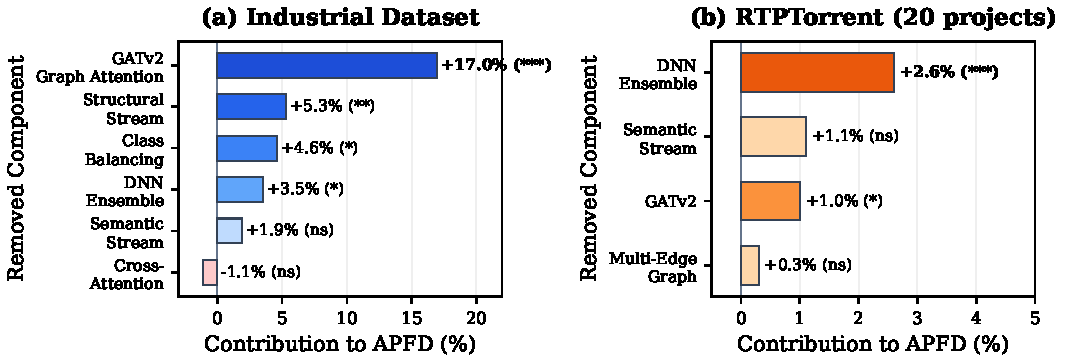
\includegraphics[width=\columnwidth]{figures/fig_ablation_crossdataset.pdf}
    \caption{Cross-dataset ablation study.}
    \label{fig:ablation_cross}
\end{figure}

%------------------------------------------------------------------------------
% RQ3: Temporal Robustness
%------------------------------------------------------------------------------

\subsection{RQ3: Temporal Validation}
\label{sec:rq3}

To evaluate how well \filopriori{} generalizes to future builds, a critical
requirement for deployment in CI environments, we conducted temporal
cross-validation on the industrial dataset. In this protocol, training data
always precedes test data chronologically, simulating a realistic deployment
scenario. We employed three validation strategies, summarized in
Table~\ref{tab:temporal_cv}.

\begin{table}[!t]
\centering
\caption{Temporal Cross-Validation Results (Industrial Dataset)}
\label{tab:temporal_cv}
\begin{tabular}{lccc}
\toprule
\textbf{Validation Method} & \textbf{APFD} & \textbf{Std} & \textbf{N} \\
\midrule
Temporal 5-Fold CV & 0.6629 & 0.279 & 215 \\
Sliding Window CV & 0.6279 & 0.272 & 248 \\
Concept Drift Test & 0.6187 & 0.277 & 152 \\
\bottomrule
\end{tabular}
\end{table}

In \textbf{Temporal 5-Fold CV}, the dataset is split into 5 chronologically
ordered folds, and each fold is used as the test set while all preceding folds
form the training set. In \textbf{Sliding Window CV}, a fixed-size window of
builds slides through time, training on the window and testing on the next
segment. The \textbf{Concept Drift Test} evaluates performance on three
temporally distant test periods to assess whether the model's effectiveness
degrades over time.

Performance degrades moderately under these stricter temporal constraints,
with APFD ranging from 0.62 to 0.66, representing a 13--19\% reduction relative to the
standard evaluation (0.7611). This decrease is expected: temporal CV uses
smaller training sets and enforces strict chronological separation, preventing
the model from exploiting co-temporal patterns. Importantly, the consistency
across all three methods (std $\leq$ 0.28) indicates that the degradation is
systematic rather than erratic, suggesting that the model's failure patterns
generalize across time periods even though overall accuracy decreases. The
concept drift test yields the lowest APFD (0.6187), but the difference from
the temporal 5-fold CV (0.6629) is modest, indicating no catastrophic
performance cliff as the temporal gap between training and evaluation data
increases.

\textbf{RTPTorrent Temporal Validation.}
To assess whether temporal robustness generalizes beyond the industrial setting,
we conducted temporal 4-fold cross-validation on all 20 RTPTorrent projects.
Each project's build history is divided into 4 chronological folds; for fold
$k$, training uses all builds before fold $k$ and testing uses the builds
in fold $k$. Table~\ref{tab:temporal_cv_rtptorrent} presents the per-project
results.

\begin{table}[!t]
\centering
\caption{Temporal 4-Fold CV Results (RTPTorrent, 20 Projects)}
\label{tab:temporal_cv_rtptorrent}
\footnotesize
\begin{tabular}{lccc}
\toprule
\textbf{Project} & \textbf{Mean APFD} & \textbf{Std} & \textbf{Folds} \\
\midrule
facebook/buck & 0.976 & 0.007 & 4 \\
apache/sling & 0.970 & 0.003 & 4 \\
eclipse/jetty.project & 0.948 & 0.018 & 4 \\
jOOQ/jOOQ & 0.924 & 0.022 & 4 \\
jsprit/jsprit & 0.923 & 0.030 & 4 \\
CloudifySource/cloudify & 0.901 & 0.023 & 4 \\
Graylog2/graylog2-server & 0.901 & 0.021 & 4 \\
jcabi/jcabi-github & 0.888 & 0.014 & 4 \\
square/okhttp & 0.882 & 0.008 & 4 \\
julianhyde/optiq & 0.872 & 0.050 & 4 \\
SonarSource/sonarqube & 0.850 & 0.014 & 4 \\
deeplearning4j/deeplearning4j & 0.842 & 0.025 & 4 \\
thinkaurelius/titan & 0.822 & 0.034 & 4 \\
doanduyhai/Achilles & 0.795 & 0.046 & 4 \\
neuland/jade4j & 0.705 & 0.021 & 4 \\
adamfisk/LittleProxy & 0.666 & 0.034 & 4 \\
DSpace/DSpace & 0.665 & 0.014 & 4 \\
l0rdn1kk0n/wicket-bootstrap & 0.620 & 0.017 & 4 \\
brettwooldridge/HikariCP & 0.599 & 0.033 & 4 \\
dynjs/dynjs & 0.563 & 0.145 & 4 \\
\midrule
\textbf{Grand Mean} & \textbf{0.816} & \textbf{0.131} & \textbf{80} \\
\bottomrule
\end{tabular}
\end{table}

The grand mean APFD under temporal CV is 0.816 (95\% CI: [0.754, 0.877]),
representing only a 2.7\% decrease from the standard evaluation (0.854).
Performance improves monotonically across folds (fold 1: 0.790, fold 2: 0.816,
fold 3: 0.823, fold 4: 0.834), indicating that \filopriori{} benefits from
additional training data without exhibiting concept drift degradation.
Fourteen of 20 projects achieve temporal CV APFD $\geq$ 0.80, and the
stability is consistent: 16 of 20 projects have cross-fold standard deviations
below 0.04.

\textbf{Cross-Dataset Temporal Synthesis.}
The temporal validation results show consistent patterns across both datasets,
with expected degradation under stricter temporal constraints. On the
industrial dataset, temporal 5-fold CV yields APFD = 0.663 (12.9\% below the
standard evaluation of 0.761). On RTPTorrent, temporal 4-fold CV yields
APFD = 0.816 (only 2.7\% below 0.854). The smaller drop on RTPTorrent
reflects the larger training sets available in multi-project evaluation. In
both cases, performance degrades smoothly across folds with no evidence
of concept drift, indicating that \filopriori{} generalizes to future builds
in both industrial and open-source settings, albeit with reduced accuracy
compared to the standard evaluation.

%------------------------------------------------------------------------------
% RQ4: Sensitivity Analysis
%------------------------------------------------------------------------------

\subsection{RQ4: Hyperparameter Sensitivity}
\label{sec:rq4}

We analyzed the sensitivity of \filopriori{} to key hyperparameters on the
industrial dataset. This analysis was conducted on the component-isolation
baseline (Table~\ref{tab:ablation_isolation}, APFD = 0.6397), not the full
model (0.7611), to isolate the effect of each hyperparameter from the
contributions of the five architectural innovations evaluated in RQ2. Each
parameter was varied while keeping others at their optimal values.
Table~\ref{tab:sensitivity} summarizes the results. We note that this
design choice means we cannot assess whether the full model (with multi-edge
graph, orphan handling, and threshold optimization) exhibits different
sensitivity patterns; the sensitivity ranges reported here apply to the
core GNN hyperparameters in isolation.

\begin{table}[!t]
\centering
\caption{Hyperparameter Sensitivity Analysis (Industrial Dataset)}
\label{tab:sensitivity}
\scriptsize
\begin{tabular}{llccr}
\toprule
\textbf{Parameter} & \textbf{Best} & \textbf{APFD} & \textbf{Worst} & \textbf{$\Delta$} \\
\midrule
Loss Function & Weighted CE & 0.6191 & 0.5834 & 3.6\% \\
Learning Rate & 3e-5 & 0.6160 & 0.5890 & 2.7\% \\
GNN Architecture & 1 layer, 2 heads & 0.6160 & 0.5890 & 2.7\% \\
Structural Features & 10 features & 0.6171 & 0.5997 & 1.7\% \\
Balanced Sampling & No balanced & 0.6154 & 0.5834 & 3.2\% \\
\bottomrule
\end{tabular}
\end{table}

The choice of loss function has the largest impact (3.6\%), with Weighted
Cross-Entropy achieving the best results on the component-isolation baseline.
In the full model, however, Focal Loss is used because it interacts more
favorably with the balanced sampler: Focal Loss's gradient modulation
($\gamma = 2.0$) complements the sampler's prior correction without
redundant class weighting, whereas Weighted CE's explicit class weights
compound with the sampler, risking over-correction (see
Section~\ref{sec:approach}). The learning rate and GNN architecture have
comparable impact (2.7\% each), with 3e-5 and a single GAT layer with 2
heads being optimal. Notably, simpler GNN
configurations consistently outperform deeper architectures (2--3 layers) and
more heads (4--8), suggesting that the test relationship graph can be
effectively captured with shallow networks and that over-parameterization leads
to overfitting on the relatively small graph structure.

The number of structural features has the smallest impact (1.7\%), with the
curated set of 10 features outperforming both the reduced (6 features) and
expanded (29 features) sets. This confirms that careful feature selection
improves generalization by reducing noise.

\textbf{RTPTorrent Sensitivity Analysis.}
To evaluate whether sensitivity patterns generalize, we conducted a
complementary analysis on all 20 RTPTorrent projects, varying three key
hyperparameters of the ensemble variant: the alpha blending coefficient
($\alpha$), the DNN training epochs, and the maximum pos\_weight clamp.
Table~\ref{tab:sensitivity_rtptorrent} presents the results.

\begin{table}[!t]
\centering
\caption{Hyperparameter Sensitivity Analysis (RTPTorrent, 20 Projects)}
\label{tab:sensitivity_rtptorrent}
\footnotesize
\begin{threeparttable}
\begin{tabular}{llcc}
\toprule
\textbf{Parameter} & \textbf{Value} & \textbf{APFD} & \textbf{$\Delta$ vs.\ Opt.} \\
\midrule
\multirow{6}{*}{$\alpha$ (GNN--DNN blend)} & 0.0 (DNN only) & 0.845 & $-$1.0\% \\
 & 0.3 & 0.854 & $-$0.0\% \\
 & 0.5 & 0.854 & $-$0.0\% \\
 & 0.7 & 0.854 & $-$0.0\% \\
 & 1.0 (GNN only) & 0.832 & $-$2.6\% \\
 & Optimized & 0.854 & -- \\
\midrule
\multirow{3}{*}{DNN Epochs} & 5 & 0.837 & $-$0.3\% \\
 & 10 & 0.843 & +0.4\% \\
 & 20 & 0.844 & +0.5\% \\
\midrule
\multirow{3}{*}{Max pos\_weight} & 10 & 0.843 & +0.5\% \\
 & 25 & 0.830 & $-$1.1\% \\
 & 100 & 0.844 & +0.5\% \\
\bottomrule
\end{tabular}
\begin{tablenotes}
\small
\item Optimized = default configuration ($\alpha$ per-project optimized, 15 DNN epochs, pos\_weight $\leq$ 50).
\item $\Delta$ vs.\ Opt.\ = relative change from optimized configuration (APFD = 0.854).
\end{tablenotes}
\end{threeparttable}
\end{table}

The $\alpha$ blending coefficient allows the framework to dynamically adapt to the data. The execution-level temporal GNN optimizations substantially improved the standalone graph performance: without the DNN ($\alpha = 1.0$), APFD drops by only $-$2.6\% (to 0.832). This confirms the ablation finding (Table~\ref{tab:ablation_rtptorrent}): the DNN ensemble still provides an additive benefit, but the model is robust to the specific choice of $\alpha$ because the structural stream can now effectively capture complex historical dependencies on its own.

DNN training epochs have marginal impact (0.8\% range). The pos\_weight
clamping exhibits a non-monotonic pattern: pos\_weight = 25 (APFD = 0.830)
slightly underperforms both pos\_weight = 10 (0.843) and pos\_weight = 100
(0.844). This behavior arises because the pos\_weight interacts with the
per-project alpha optimization: a different pos\_weight changes the DNN's
output distribution, which in turn shifts the optimal $\alpha$ for each
project, producing non-linear aggregate effects. The overall range remains
narrow (1.6\%), confirming that \filopriori{} is not sensitive to these
hyperparameters in the open-source setting.

\textbf{Cross-Dataset Sensitivity Synthesis.}
The sensitivity analyses on both datasets confirm that \filopriori{} is robust
to hyperparameter choices. On the industrial dataset, the maximum sensitivity
range is 3.6\% (loss function); on RTPTorrent, the maximum range is 2.6\%
(observed when disabling the DNN via $\alpha = 1.0$). Overall, the
architectural choices (such as the temporal GNN structure) are more impactful
than the specific values of continuous hyperparameters.

%------------------------------------------------------------------------------
% Summary of Experimental Results
%------------------------------------------------------------------------------

\subsection{Summary of Results}
\label{sec:results_summary}

Table~\ref{tab:results_summary} summarizes \filopriori{}'s performance across
all experimental settings.

\begin{table}[!t]
\centering
\caption{Summary of Experimental Results}
\label{tab:results_summary}
\scriptsize
\begin{tabular}{lccr}
\toprule
\textbf{Setting} & \textbf{APFD} & \textbf{vs.\ Best} & \textbf{vs.\ Weakest} \\
\midrule
Industrial\textsuperscript{a} & 0.761 & +10.2\% & +27.6\% \\
RTPTorrent\textsuperscript{b} & 0.854 & +1.6\% & +23.5\% \\
\bottomrule
\end{tabular}
\begin{tablenotes}
\small
\item APFD: Average Percentage of Faults Detected (higher is better).
\item \textsuperscript{a} Full architecture with multi-edge graph (5 edge types).
\item \textsuperscript{b} Ensemble variant with co-failure graph + DeepOrder DNN blending (Section~\ref{sec:ensemble}).
\end{tablenotes}
\end{table}

The experimental results demonstrate that \filopriori{} achieves
state-of-the-art performance across both industrial software testing (0.761)
and open-source CI/CD environments (0.854), using two distinct
configurations tailored to the available metadata
(Table~\ref{tab:rtptorrent_config}). On the industrial dataset, the full
graph-based architecture with multi-edge graph (\textsc{Filo-Priori-Full})
outperforms all five deep learning baselines by statistically significant
margins ($p < 0.001$). On RTPTorrent, the ensemble variant
(\textsc{Filo-Priori-Ensemble}) achieves the highest aggregate APFD, leading
in 11 of 20 projects; after Holm-Bonferroni correction, improvements over
NodeRank and RETECS remain statistically robust, while the narrower margins
over TCP-Net, FailRank-BB, and DeepOrder should be interpreted with caution.
The two variants reveal complementary strengths:
graph-based structural modeling drives performance on the industrial dataset,
while the DNN ensemble provides crucial complementary signal on RTPTorrent.
